It is not surprising that weather conditions directly impact the wind power generation. The typical input parameters for wind power prediction are wind speed, air density, temperature and pressure \cite{WindPowerGenerationUsingANN} with the most influential factor being wind speed because it is directly converted to power in the wind turbine. The following subsections will describe the parameters relationship to wind production and how it is used in the modelled ANN.

\subsubsection{Wind Speed}
The relationship between hourly wind speed and hourly wind power production of DK1 is seen in Figure~\ref{fig:windVsProd}. The graph clearly shows the expected impact of wind speed on the wind energy production.

\begin{figure}[h!]
\centering
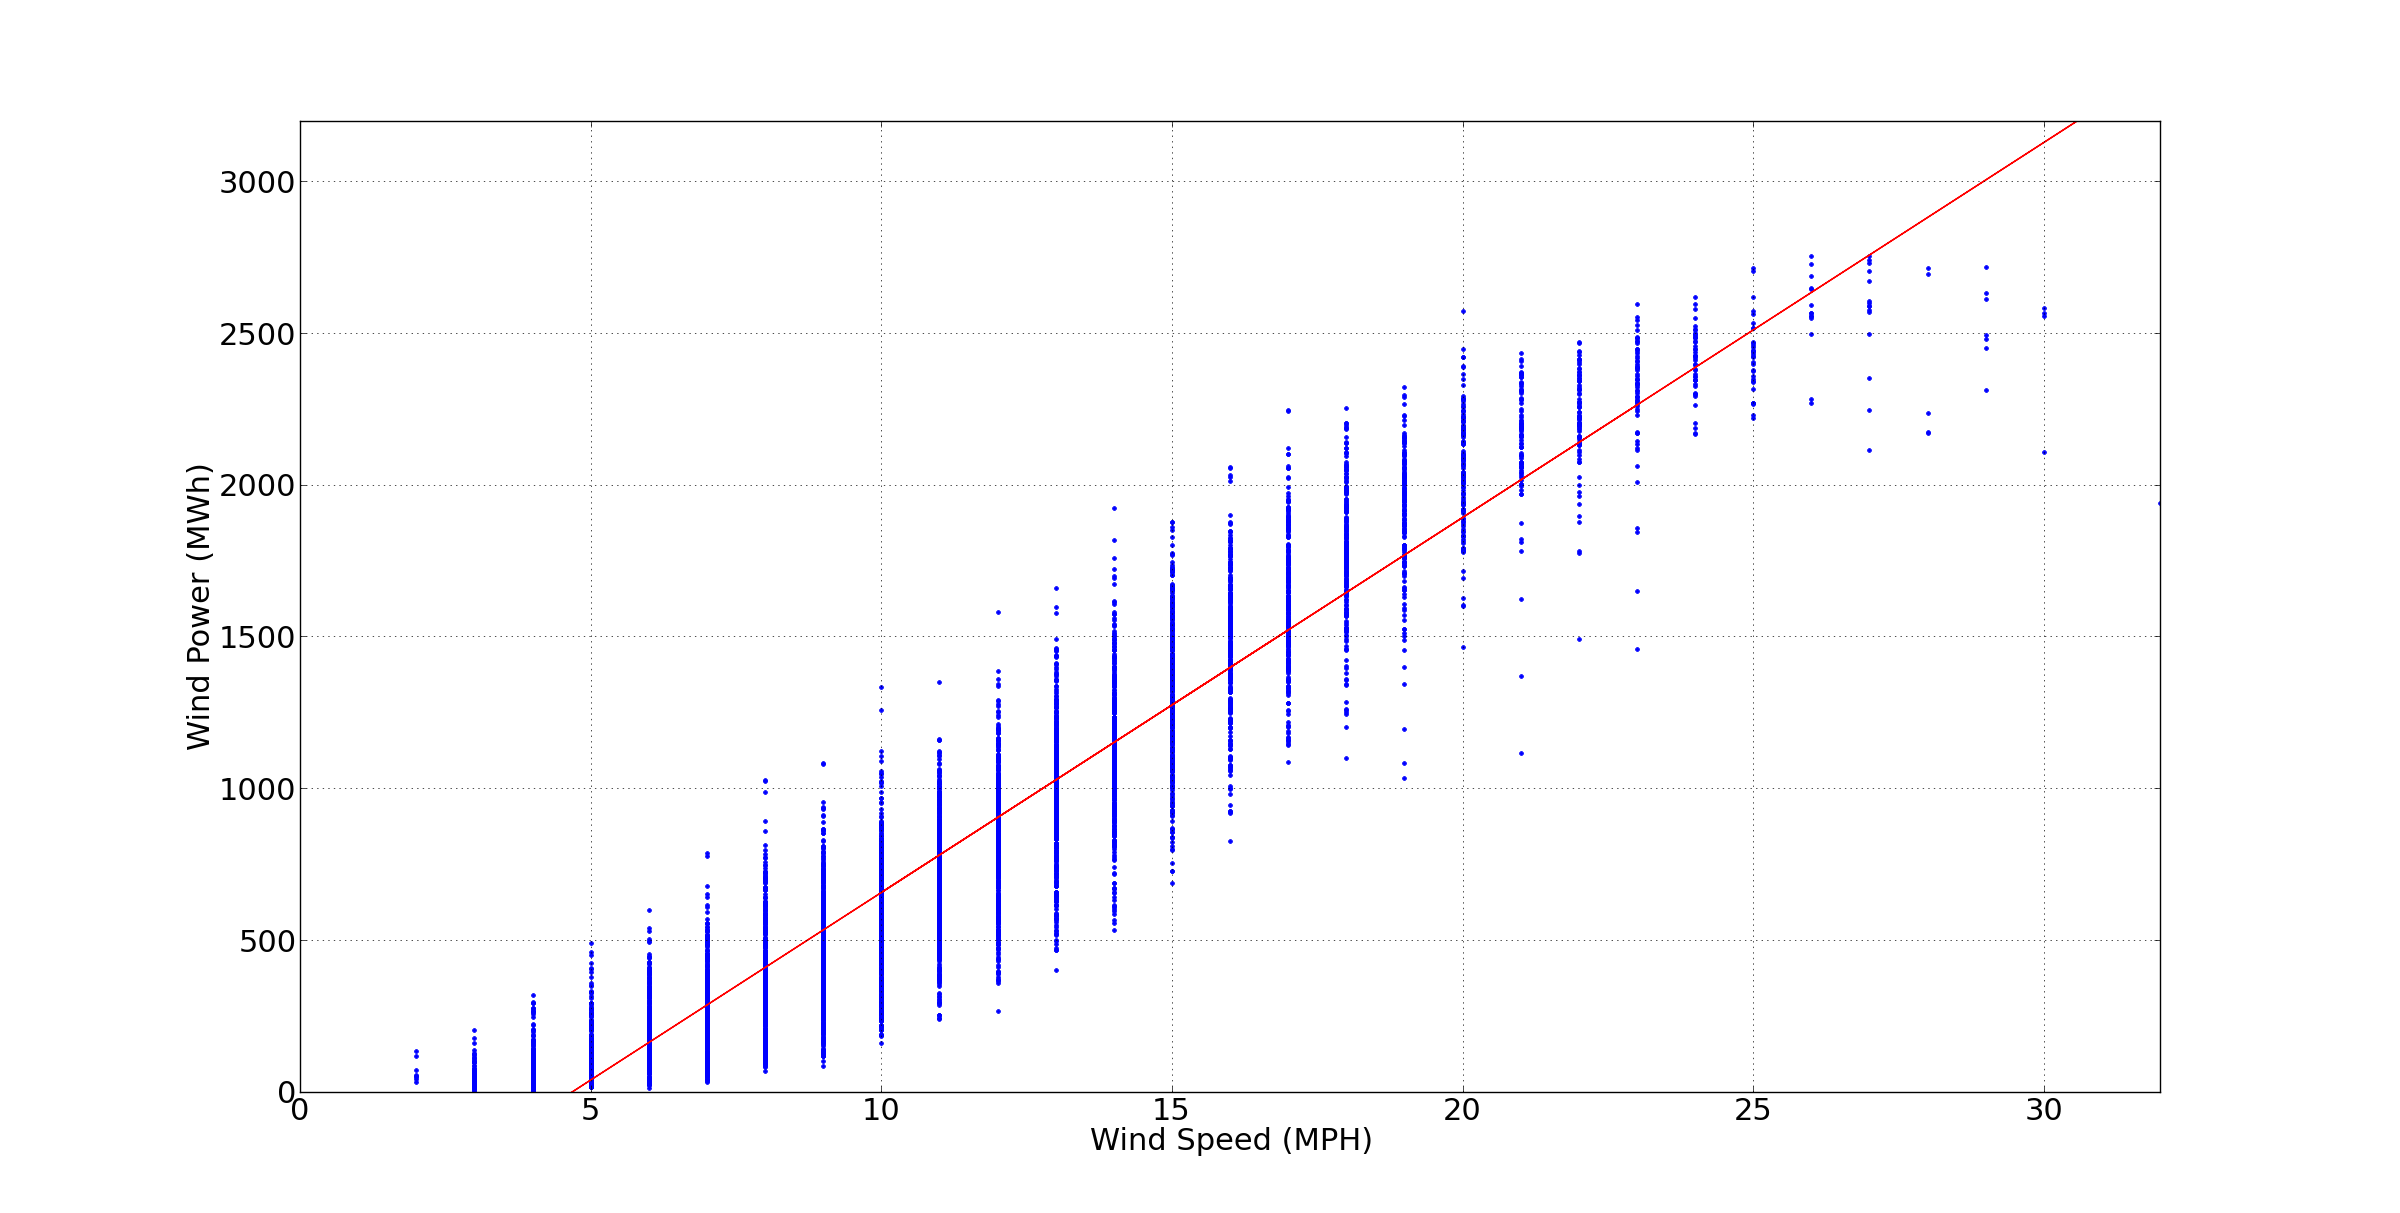
\includegraphics[width=0.99\linewidth,natwidth=898,natheight=587]{billeder/WindSpeedVsProduction.png}
\caption{Wind speed vs. wind production in 2012}
\label{fig:windVsProd}
\end{figure}

\subsubsection{Air Density}
It is described in the Wind Power Production section that wind power is proportional to air density where a higher density means more power. Furthermore, air density depends directly on temperature and pressure which can be described by $Air Density=\frac{P}{(R*T)}$ where R is a gas constant. If pressure decreases so will air density and therefore it is expected that the wind power production will be less during periods with lower pressure. This can best be illustrated by finding days with same wind speed and showing that production will have a tendency to decrease when the pressure is lower. This is illustrated in Figure~\ref{fig:pressureVsProd} where all days with wind speed 13 is selected. What is noticeable from all pressure data is the low range which goes from 980 to 1030 (SHOW PLOT WITH THAT).
The formula expresses that when the temperature decreases the air density will increase linearly e.g. the wind power production will be higher in times of low temperature. This exact relationship is seen in Figure~\ref{fig:tempVsProd}.
\begin{figure}[h!]
\centering
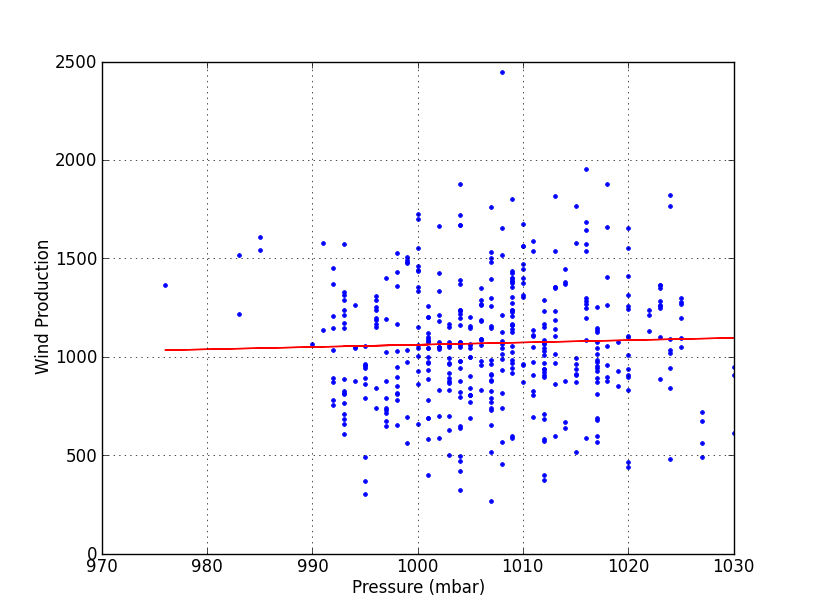
\includegraphics[width=0.99\linewidth,natwidth=898,natheight=587]{billeder/windProductionForPressure13.png}
\caption{Pressure vs. wind production in 2012}
\label{fig:pressureVsProd}
\end{figure}

\begin{figure}[h!]
\centering
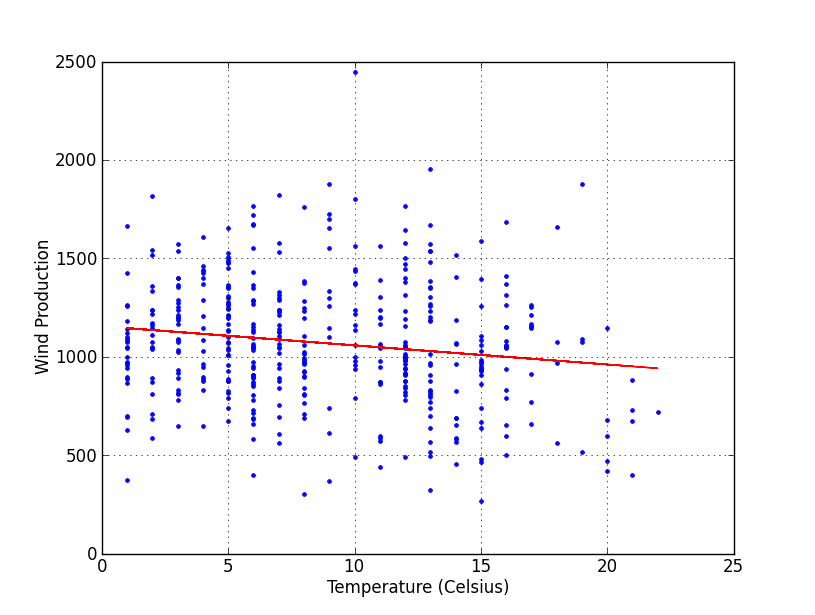
\includegraphics[width=0.99\linewidth,natwidth=898,natheight=587]{billeder/windProductionForTemperature13.png}
\caption{Temperature vs. production in 2012}
\label{fig:tempVsProd}
\end{figure}

SHOW figure with air density.

\subsubsection{Wind Direction}
bla bla intro. Figure~\ref{fig:windDirVsProd} shows that western wind has a tendency to produce more energy. (need to further investigated but seems valid when looking at dk).
\begin{figure}[h!]
\centering
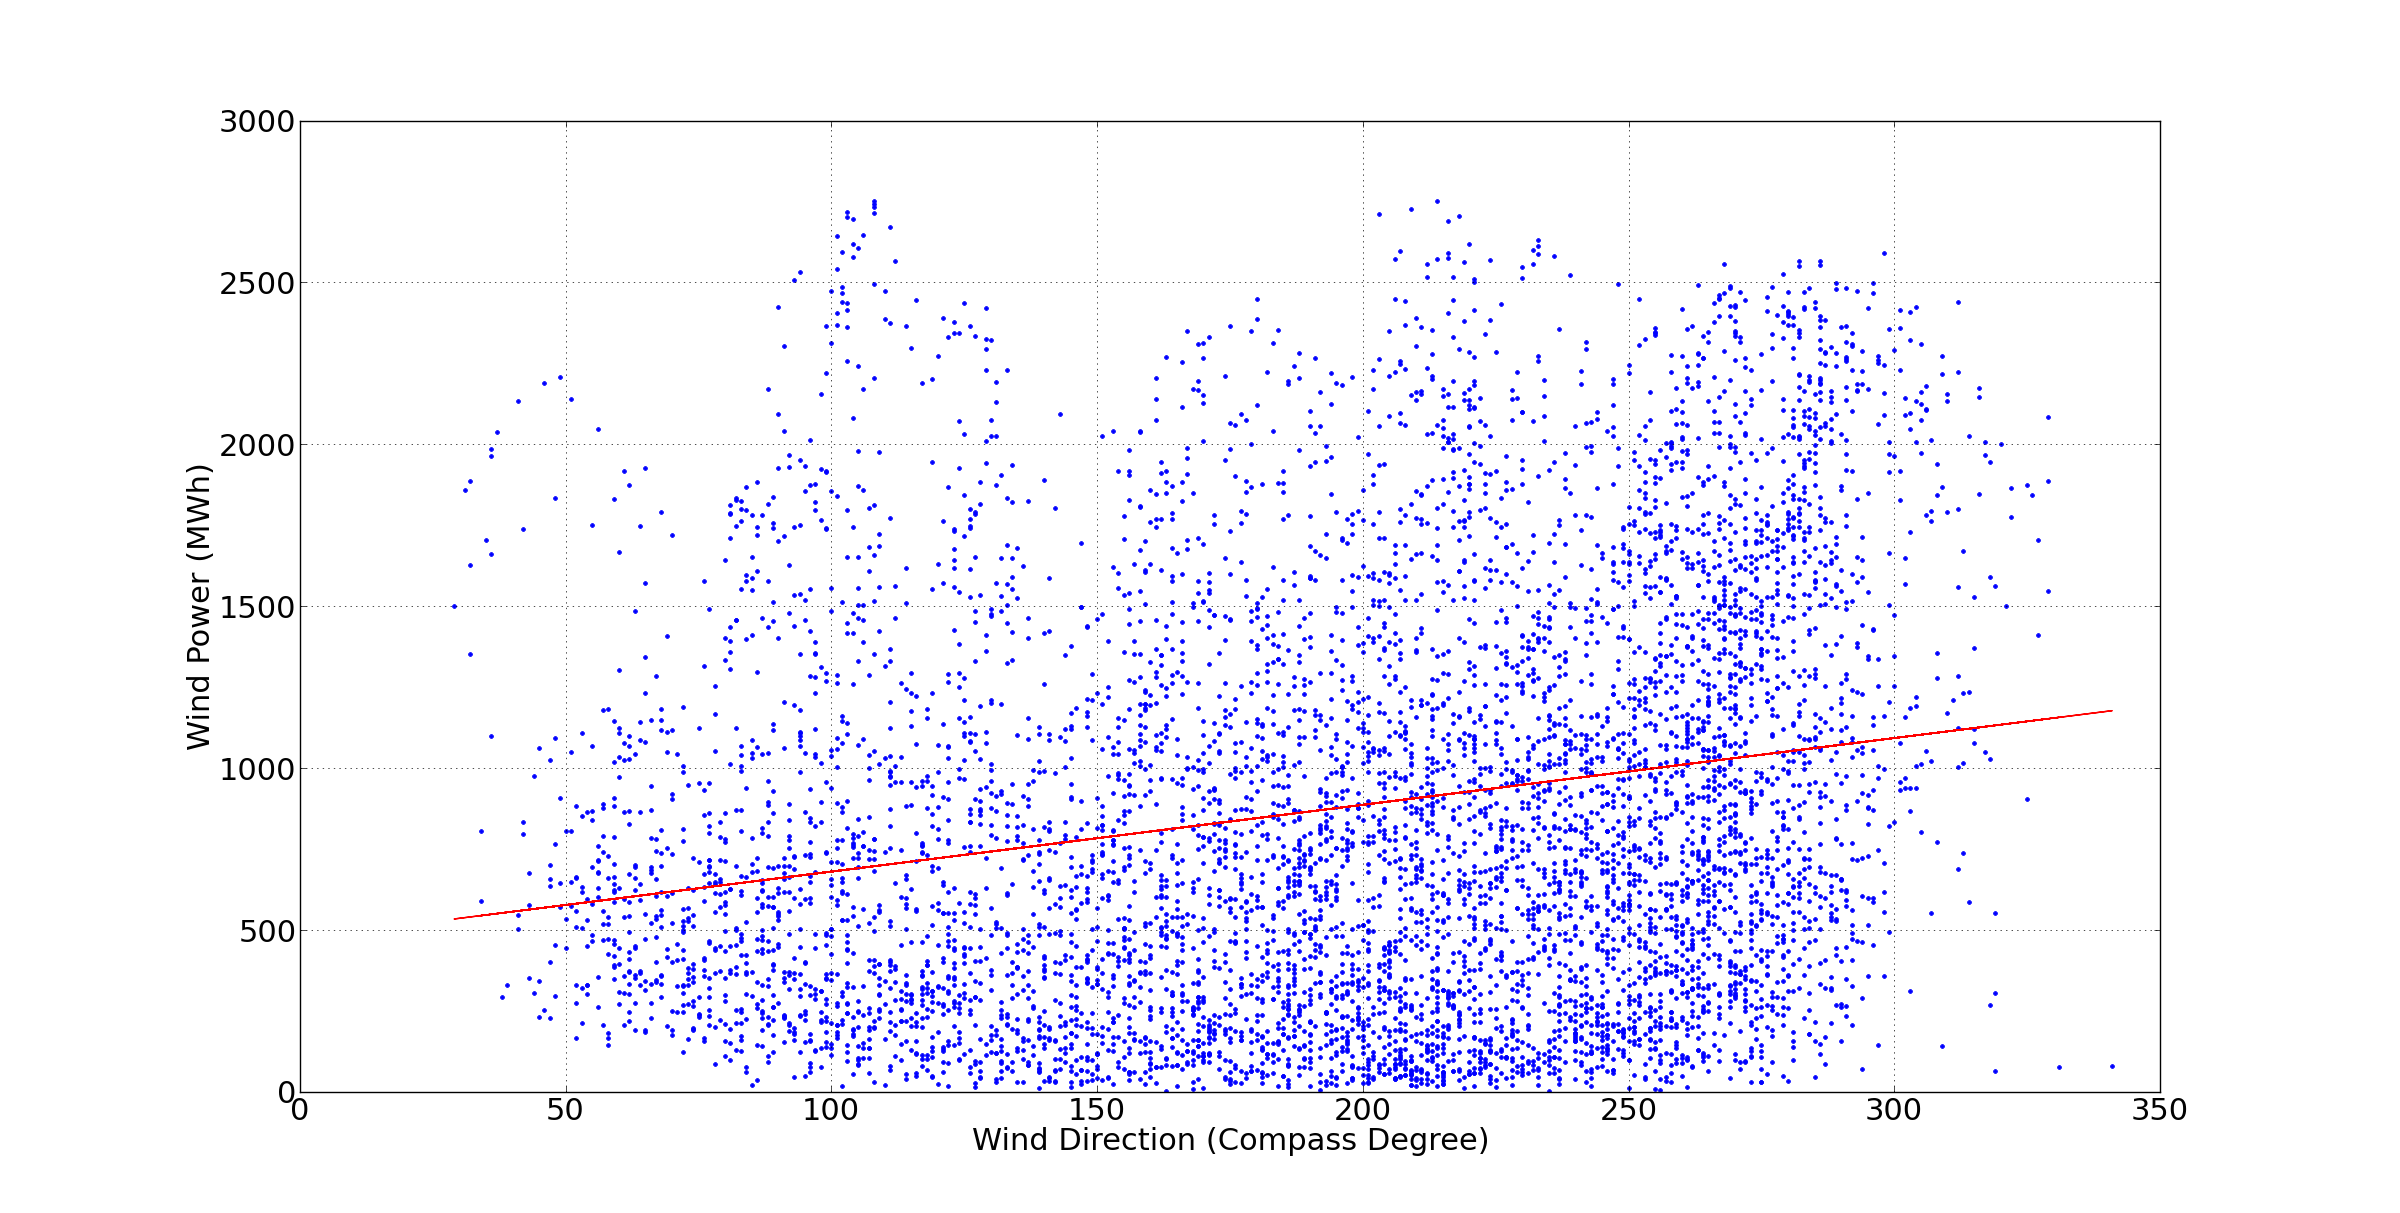
\includegraphics[width=0.99\linewidth,natwidth=898,natheight=587]{billeder/productionVsWindDirection.png}
\caption{Wind Direction vs. wind production in 2012}
\label{fig:windDirVsProd}
\end{figure}

\subsubsection{Relative Humidity}
The dew point is a water-to-air saturation temperature. The dew point is associated with relative humidity. A high relative humidity indicates that the dew point is closer to the current air temperature. Relative humidity of 100\% indicates the dew point is equal to the current temperature and that the air is maximally saturated with water. When the dew point remains constant and temperature increases, relative humidity decreases.[1]

\subsection{Modelling Artificial Neural Network}
The ANN will be trained with input the hourly parameters of wind speed, temperature, pressure and humidity and then compared to the actual production of that hour.

Black art --- experimenting with hidden layers, momentum and learning rate. 